%
% path-finding user interfaces
% @author Tobias Weber <tweber@ill.fr>
% @date july-2021
% @license see 'LICENSE' file
%

\chapter{User Interfaces}
\label{ch:gui}

The software has been realised in a modular fashion, it comprises a core
and a library module (see chapter \ref{ch:impl}), which can be easily linked 
into external C++ applications. Such a library usage will be important in the
future when we plan to utilise the software as a plug-in module to the instrument
control software \textit{NOMAD} \cite{web_NOMAD} that is employed at the Institut 
Laue-Langevin.

Furthermore, a graphical user interface (GUI) has been implemented for a visual
and interactive representation of the instrument and the underlying algorithms.
The GUI is described in detail in section \ref{sec:gui}.

Finally, the software allows scripting via \textit{Python} \cite{Rossum2011, web_python}. 
Apart from simply setting up a workflow and plotting the results, the \textit{Python}
interface will allow the usage of the software in \textit{Python}-based instrument
control systems such as \textit{NICOS} \cite{web_NICOS}, which is used at the 
Forschungsreaktor M\"unchen II (FRM-II). 
Details on the scripting interface can be found in section \ref{sec:scripting}.





\section{Graphical User Interface}
\label{sec:gui}

The software's main graphical user interface (GUI), as it is depicted in Fig. \ref{fig:gui},
is based on the \textit{Qt} framework \cite{web_Qt}, which allows for an easy and rapid
cross-platform GUI development in \textit{C++}. We support both current releases of \textit{Qt},
namely version 5 and version 6.


\begin{figure}[htb]
		\begin{center}
			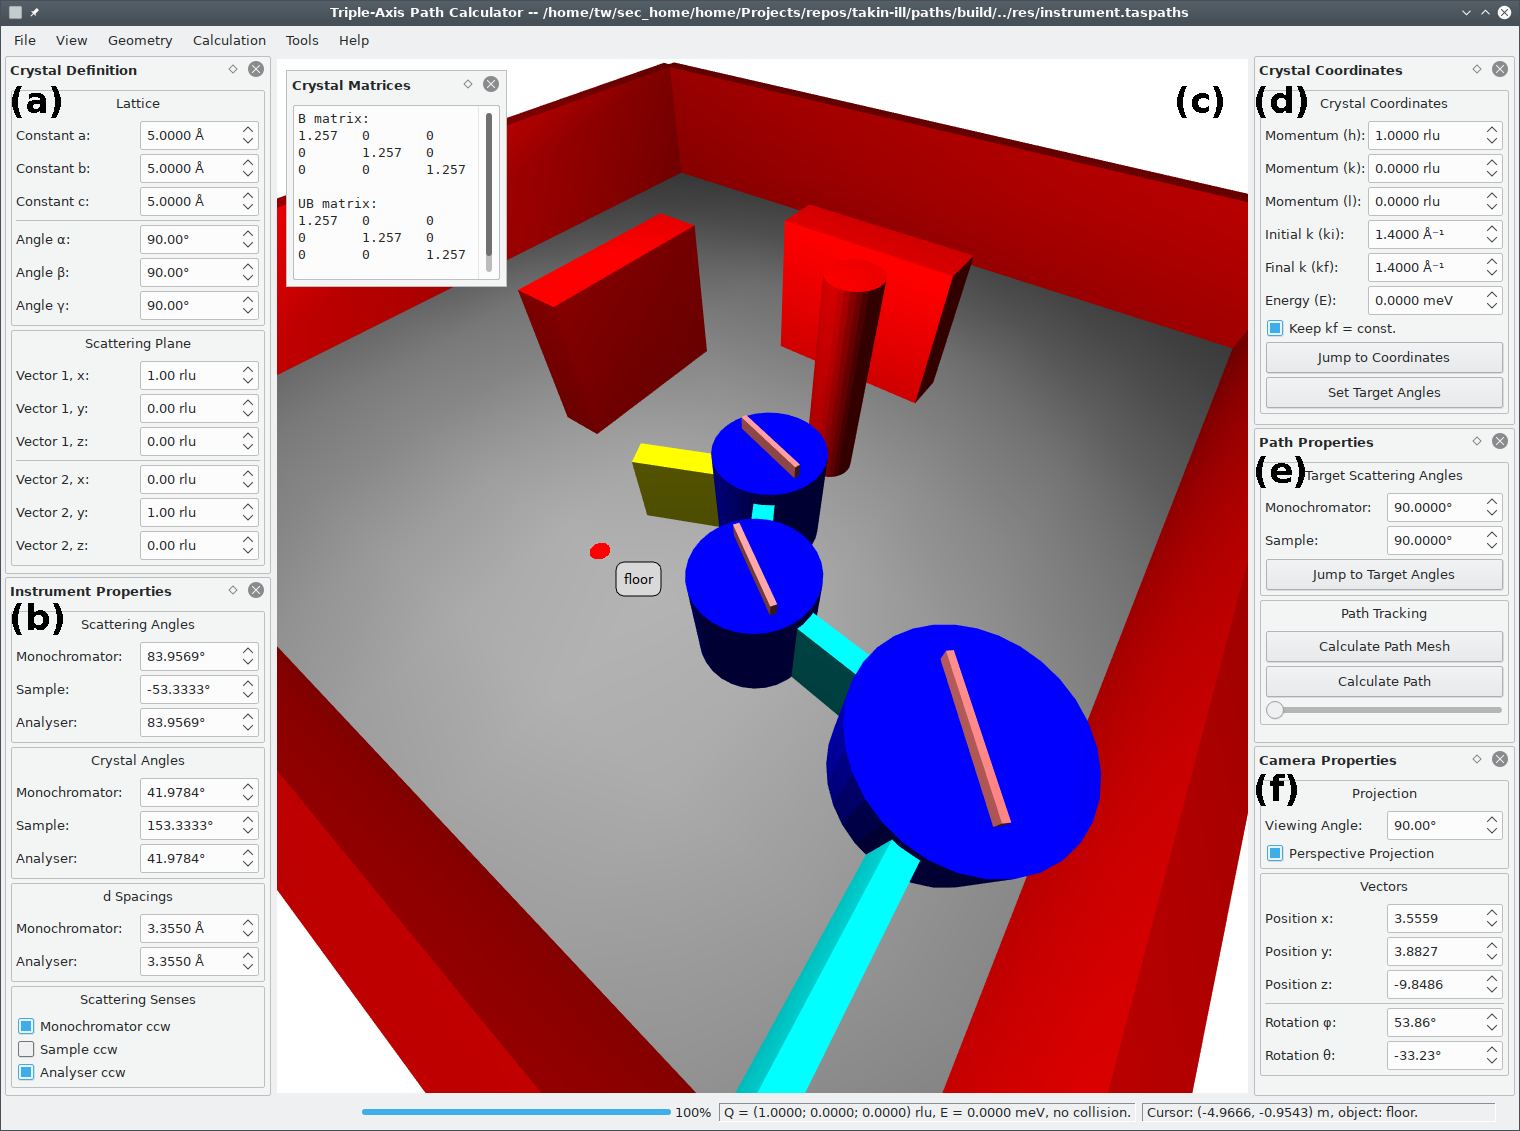
\includegraphics[width = 1 \textwidth]{figures/gui}
		\end{center}
	\caption{Main GUI. Here, instrument and sample crystal properties can be set up,
		walls can be added and moved and paths around them be calculated.
		The central view provides a three-dimensional visualisation of the instrument
		configuration and is fully dynamic: Every element, including the instrument
		and the wall segments, can be moved or manipulated using the mouse.
		\label{fig:gui}}
\end{figure}



\begin{figure}[htb]
		\begin{center}
			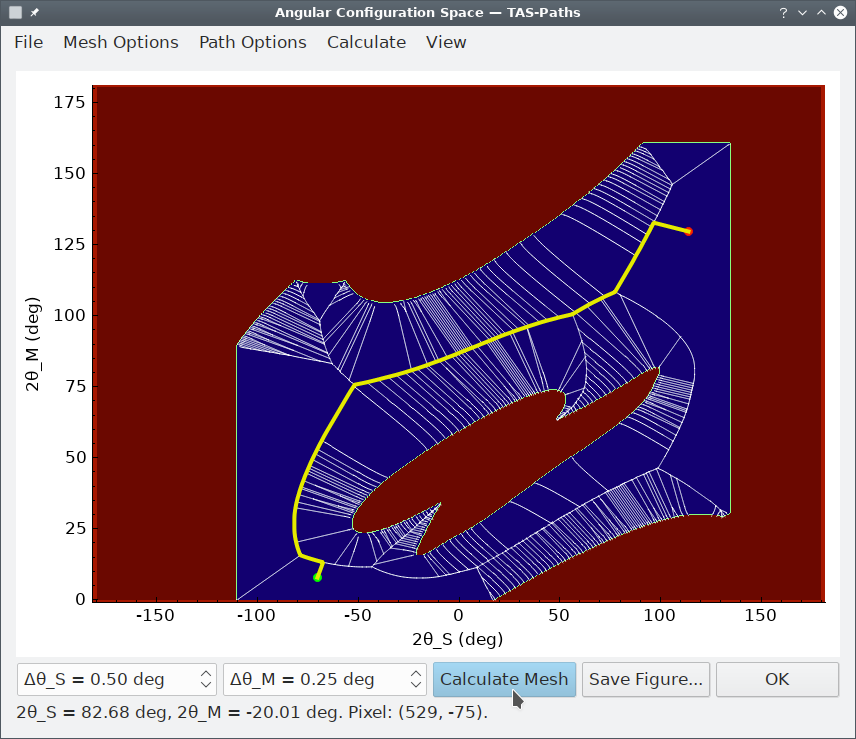
\includegraphics[width = 0.66 \textwidth]{figures/gui_configspace}
		\end{center}
	\caption{Angular configuration space and path calculation. The figure plots all
	possible instrument positions for the monochromator and sample scattering angles,
	$2\theta_M$ and $2\theta_S$, respectively. Forbidden positions are shown in red.
	These can be invalid angles as well as collisions of the instrument with walls
	(here, specifically, the pillar from Fig \ref{fig:gui}), or with itself.
	Allowed positions are drawn in blue. The mesh of all possible instrument
	paths is shown as white lines, while a currently selected example path from
	the red start to the green target position is shown as a yellow line.
		\label{fig:gui_configspace}}
\end{figure}




\section{Python Scripting Interface}
\label{sec:scripting}
